% this file is called up by thesis.tex
% content in this file will be fed into the main document

%: ----------------------- name of chapter  -------------------------
\chapter{Teori} % top level followed by section, subsection
\label{teori}

%: ----------------------- paths to graphics ------------------------
\ifpdf
    \graphicspath{{3_theory/figures/PNG/}{3/figures/PDF/}{3/figures/}}
\else
    \graphicspath{{3_theory/figures/EPS/}{3/figures/}}
\fi

\graphicspath{{3_theory/figures/}{3/figures/}}

%: ----------------------- contents from here ------------------------

\section{Problemet med skadegörelse}

Sannolikheten för vandalisering av busshållplatser ökar när det är mörkt ute och under nattetid just på grund av att brottet inte skall upptäckas. Det har visat sig att i ett område där det finns en skylt som säger att området är övervakat har brottsligheten minskat och människors uppförande förbättrats.\\ 

Brottsförebyggande rådet (BRÅ) skriver på sin hemsida att kameraövervakning i brottsförebyggande syfte blir allt mer vanligt i Sverige. Speciellt när kameraövervakningslagen trädde i kraft i juli år 2013. Lagändringen har underlättat för installationer av kameraövervakningssystem. 

\begin{figure}[h]
  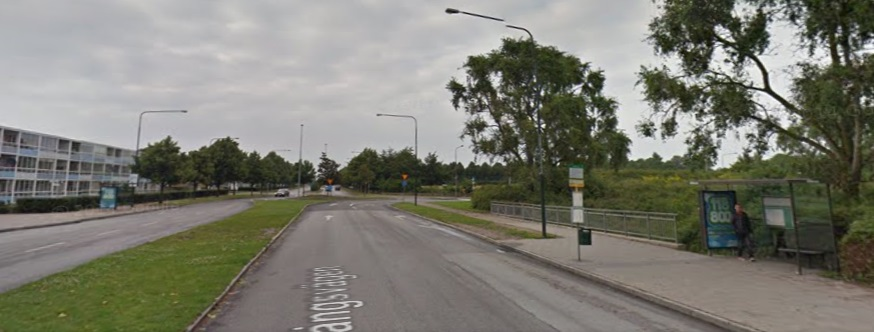
\includegraphics[width=\linewidth]{lind.jpg}
  \caption{En obevakad hållplats i Malmös stadsdel Lindängen. (Google Maps: Lindängen - Malmö)}
  \label{fig:lind}
\end{figure}

Busshållplatser i utsatta områden utan övervakning där människor passerar utsätts för skadegörelse och denna skadegörelse kostar samhället pengar. Skadegörelsen fortsätter än idag eftersom det inte finns några bra lösningar för att hantera problemet med skadegörelse. Detsamma gäller tryggheten omkring de busshållplatser som är utsätta för vandalisering.\\

En busshållplats som är övervakad dygnet runt är en ineffektiv lösning. Övervakningen ska ske i samband med att specifika villkor är uppfyllda. Villkoren för aktiv övervakning är då en människa är närvarande, rörelse registreras eller vandalisering mot busshållplatsen utförs. Om inget villkor är uppfyllt så kommer systemet att vara i ett passivt tillstånd och enbart lyssna på förändringar.\\

Sensorer används för att lyssna till förändringar hos omgivningen. Dessa förändringar kommer att utvärderas och jämföras med fördefinierade villkor för när övervakningssystemet ska aktiveras. När ett villkor är uppfyllt så kommer systemet att aktiveras och börja registrera data och skicka denna data via internet till en server för datalagring.\\

% ---------------------------------------------------------------------------
%: ----------------------- end of thesis sub-document ------------------------
% ---------------------------------------------------------------------------

